
% this file is called up by thesis.tex
% content in this file will be fed into the main document

%: ----------------------- introduction file header -----------------------
\begin{savequote}[50mm]
Now this is not the end. It is not even the beginning of the end. But it is, perhaps, the end of the beginning. 
\qauthor{Winston Churchill}
\end{savequote}


\chapter{Conclusiones y trabajo futuro}
\label{cha:Conclusions}

% the code below specifies where the figures are stored
\ifpdf
    \graphicspath{{6_conclusion/figures/PNG/}{6_conclusion/figures/PDF/}{6_conclusion/figures/}}
\else
    \graphicspath{{6_conclusion/figures/EPS/}{6_conclusion/figures/}}
\fi


En este capítulo se presentan las conclusiones de este trabajo de investigación. Además se comentan los trabajos futuros que se pueden realizar para continuar esta línea de investigación.

%------------------------------------------------------------------------- 

\section{Conclusiones}

En esta tesis doctoral se ha presentado el método DBA y se ha propuesto su utilización para la evaluación de competencias genéricas. El método DBA tiene su origen en la metodología DBR y se basa en el diseño de evaluaciones a partir de indicadores de la actividad de los estudiantes generada en los entornos virtuales de apoyo a la docencia. El diseño de evaluaciones se realiza dentro del ciclo de contraste de hipótesis. De esta forma, un docente que quiera realizar una evaluación formula un diseño (hipótesis de evaluación) a partir de los indicadores del entorno virtual, el sistema devuelve los resultados de aplicar esta fórmula y el docente evalúa su validez para la evaluación de la competencia. Mientras no le sean válidos, el docente seguirá rediseñando la fórmula de evaluación hasta alcanzar un diseño que le satisfaga o hasta que tenga que descartar los resultados.

Para poner en práctica el método DBA se han propuesto herramientas de tipo DSL. En primer lugar se desarrolló SASQL, un DSL para obtener indicadores de la actividad de los estudiantes del VLE y EvalCourse, el software que interpreta las consultas escritas en SASQL. En segundo lugar se desarrolló VWQL, DSL que en este caso obtiene indicadores de la activdad de los estudiantes de los mundos virtuales y EvalSim, el software que interpreta las consultas escritas en VWQL.

Se han desarrollado seis estudios de caso entre los cursos 2010-11 y 2014-15 en el que los docentes han utilizado los DSL que implementan el método DBA para la evaluación de competencias genéricas. Estas experiencias han servido para obtener retroalimentación de los docentes que han participado. Además, estos estudios de caso se han presentado en varios congresos y revistas, pasando por procesos de revisión ciega por pares.

De entre los participantes en estos estudios de caso y otros contextos educativos se ha llevado a cabo una encuesta para llevar a cabo la evaluación del método. En primer lugar, con esta encuesta se ha dado validez al método para ser utilizado en la evaluación de diferentes competencias genéricas. Los indicadores han sido aceptados como válidos para evaluar competencias genéricas por un porcentaje alto de docentes para cada competencia genérica. Además, aquellos docentes que no consideraron la evaluación de alguna competencia lo hicieron porque consideraban que el indicador debería ser completado con más información. Asimismo, mediante la formulación de diferentes hipótesis nulas se ha demostrado que las respuestas de los participantes en la encuesta son independientes tanto de los conocimientos de programación (nulos o básicos frente a medios o avanzados) como de la relación de los participantes con la docencia (profesorado universitario, profesorado no universitario o no profesorado relacionado con las wikis).

Por tanto, de los resultados de la evaluación realizada, se considera que la metolodogía DBA parece ser una propuesta eficaz para abordar la evaluación de competencias genéricas, ya que aporta indicadores objetivos del trabajo de los estudiantes en las herramientas virtuales, indicadores que han sido aceptados por los docentes para la evaluación de competencias genéricas y cuya obtención mediante las herramientas proporcionadas no les requiere conocimientos informáticos avanzados.


% ----------------------------------------------------------------------

\section{Trabajo futuro}

Durante la realización de este trabajo se han superado los retos que se plantearon inicialmente. Sin embargo, durante la realización de la misma, se han encontrado algunos problemas o nuevos retos que no han llegado a ser abordados pero que complementarían en muchos casos esta tesis doctoral.

Estos trabajo futuros serían:
\begin{itemize}
\item Añadir indicadores basados en la aplicación de técnicas del análisis de las redes sociales (SNA) a los entornos virtuales de aprendizaje. En un wiki de Moodle utilizado en clase se puso a los estudiantes en parejas para que cada pareja realizase su trabajo en una página del wiki. Una vez finalizada la actividad, aplicando técnicas de SNA se obtuvo el grafo~\ref{fig:SNAWiki}. En dicho grafo, el nodo del medio es el profesor. Puede verse como al principio el profesor creó la sección principal, mientras que los estudiantes ubicaron los enlaces a sus páginas en dicha página principal (arista que une a los nodos periféricos con el nodo central). El resto de arista que une normalmente dos nodos periféricos representa los estudiantes que colaboraron juntos en una página. El tamaño de los nodos representa la cantidad de trabajo realizado por cada estudiante.
\item Integrar los DSL con los propios entornos virtuales de aprendizaje. En este momento las herramientas virtuales (VLE, wiki o mundo virtual) funcionan por su lado. Los DSL se conectan a ellos de algún modo y se obtienen los indicadores. Sería interesante poder integrar el DSL en dichas herramientas dentro del perfil de supervisor que se otorga a los docentes en muchas de estas herramientas virtuales.
\item Establecer una biblioteca que relacione actividades a realizar por los estudiantes en los entornos de aprendizaje, indicadores que se generan y competencias genéricas que se evaluarían con dichos indicadores.
\end{itemize}

\begin{figure}
  \begin{center}
    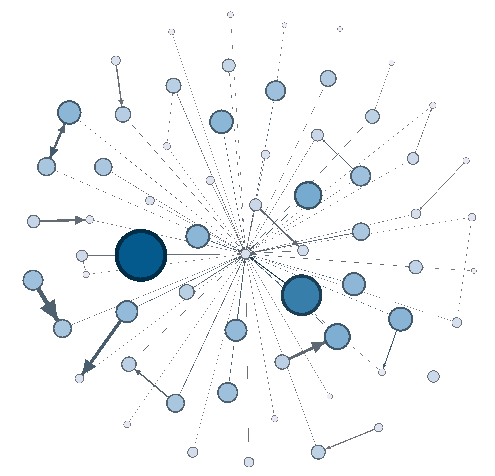
\includegraphics[scale=0.5]{SNA-Grafo-Wiki-SD.png}
  \end{center}
  \caption{Grafo resultante de aplicar técnicas de SNA a un wiki de Moodle}
  \label{fig:SNAWiki}
\end{figure}

% ----------------------------------------------------------------------